%%%%%%%%%%%%%%%%%%%%%%%%%%%%%%%%%%%%%%%%%%%%%%%%%%%%%%%%%%%%%%
% NUbots' TDP 2017
%
% Date: 24.11.2016
%
%
\documentclass{llncs}
%
\usepackage{graphicx}
\usepackage[colorinlistoftodos]{todonotes}
\usepackage{verbatim}
%
\begin{document}
%

\frontmatter          % for the preliminaries
%
\pagestyle{headings}  % switches on printing of running heads
\addtocmark{The NUbots Qualification material for RoboCup 2019} % additional mark in the TOC
%
%
\mainmatter              % start of the contributions
%
\title{The NUbots Team Description Paper 2019}
%
\titlerunning{The NUbots Team Description for 2019}  % abbreviated title (for running head)
%                                     also used for the TOC unless
%                                     \toctitle is used

\author{Matthew Amos
        \and Alex Biddulph
        \and Stephan Chalup
        \and Daniel Ginn
		\and Alexandre Mendes
        \and Josephus Paye
        \and Ysobel Sims
        \and Peter Turner
        \and Taylor Young
        }
       
%
\authorrunning{Amos et al.}   % abbreviated author list (for running head)
%
%%%% modified list of auth for the TOC (add the affiliations)
\tocauthor{
M. Amos,
A. Biddulph,
S. Chalup,
D. Ginn,
A. Mendes,
J. Paye,
Y. Sims,
P. Turner,
T. Young
}

%
\institute{Newcastle Robotics Laboratory\\ School of Electrical Engineering and Computing\\
Faculty of Engineering and Built Environment\\
The University of Newcastle, Callaghan 2308, Australia\\
Contact: \email{nubots@newcastle.edu.au}\\
Homepage: \url{http://robots.newcastle.edu.au}}
%

\maketitle              % typeset the title of the contribution


\begin{abstract}
The NUbots are the RoboCup team of the University of Newcastle, Australia. In 2019 they continue their participation in the Teen-Size Humanoid League using their self-printed robots based on the Igus-Nimbro design. In previous years, the NUbots participated in the Standard Platform League (2002-2011) and the Kid-Size Humanoid League (2012-2017). This year, the NUbots have participated in the Teen-Size Humanoid League, achieving third place. The NUbots' research addresses applications of machine learning, software engineering and computer vision. Their current research focus is Deep Learning. This paper provides an overview of the NUbots team, its software system and robot platform.
\end{abstract}

%
\section{Introduction}
For 16 years the Newcastle Robotics Laboratory has been hosting the NUbots robot soccer team as its central project. The NUbots previously competed at RoboCup in the Four-Legged League, the Standard Platform League and, until 2017, in the Kid-Size Humanoid League. In 2018, the NUbots debuted in the Teen-Size Humanoid League where they placed third. In 2019, the NUbots will be continuing their involvement in the Teen-Size Humanoid League.

The goal of the 2019 NUbots team is to improve upon their 2018 performance with further modifications to their NUgus robot design and the software. The NUgus robot is based on the Igus-Nimbro design developed by the University of Bonn~\cite{allgeuer2016igus}. 

The following sections describe research and history of the NUbots team. Some of the material, such as the history and previous research, was already covered by~\cite{AmosEtAl2018}.


\section{Scientific Aspects of the NUbots team}
 
The scientific aspects of the current NUbots system involve the implementation of deep learning on robots, software engineering for robotics and AI, and various aspects of computer vision, localisation, human-robot interaction and machine learning.

\subsection{Current Research Projects in the Newcastle Robotics Lab}
Some ome of the NUbots' current projects are listed below. Additional details on the NUbots research in the past 16 years can be found in~\cite{AmosEtAl2018} and on the NUbots homepage.\\

\noindent\textbf{Stereo Visual Mesh:} 
Recent work in the lab has resulted in the development of a high framerate obstacle detector, named The Visual Mesh~\cite{Houliston2018VisualMR}. The Visual Mesh, used in conjunction with deep learning, is capable of detecting a soccer ball in a $1280\times 1024$ image at framerates of up to $400$ fps on a humanoid robot, with little loss of accuracy when the ball is at distance. Current research being developed by a PhD student aims at increasing the detection capabilities of the Visual Mesh by considering multiple objects, distance, and stereo vision.\\

\noindent\textbf{Localisation Techniques for Robotics:} 
Another PhD research project is using fast Deep Learning algorithms to semantically label important navigational features to enhance visual SLAM implementations like ORB-SLAM \cite{mur2015orb}. Preliminary tests of ORB-SLAM have demonstrated that it is capable of running in real-time on our CPU while the NUgus is walking on the field, and is able to maintain tracking under the swaying and jarring motions of humanoid locomotion. The results of this testing will be presented at the AI2018 conference in New Zealand\footnote{AI 2018: \url{https://ecs.victoria.ac.nz/Events/AI2018/}}. We believe that ORB-SLAM will be able to provide localisation where visual odometry methods tested by NimbRo~\cite{Nimbro2018TDP} proved unsuitable.\\

\noindent\textbf{Multi-Objective Evolutionary Algorithms for Walk Optimisation:} 
The NUbots walk engine and kick scripts were optimised by a Software Engineering Honours student using a Multi-Objective Evolutionary Algorithm (MOEA). The Gazebo simulation engine~\cite{koenig2004design} was used to allow rapid optimisation without causing undue wear and tear on the physical robots. A generic MOEA framework was implemented and utilised the Ignition Transport library\footnote{Ignition Web: \texttt{https://ignitionrobotics.org/libs/transport}} to communicate with the Gazebo simulation engine. 

When tested on the robot, the resulting script doubled the kick distance, without the robot falling over afterwards. Moreover, the robot's torso sway during the kick process was decreased by 50\%. The MOEA framework was also tested on the walk engine, increasing the walk speed by 30\%, and its stability by 40\%. Further work on this system will improve the accuracy of the simulated servos as well as implementing more advanced learning techniques.\\

\noindent\textbf{Semi-Synthetic Data Generation:} 
A Physics-Based Rendering (PBR) pipeline has been developed to generate semi-synthetic data for deep learning purposes as part of a PhD project. The PBR generation tool utilises $360^{\circ}$ High Dynamic Range (HDR) images to create realistic lighting for the constructed scene. Soccer balls, goals and the soccer field are synthetically generated, allowing the random placement of camera positions within the scene to create a large quantity of fully annotated semi-synthetic data.

The pipeline is capable of exporting either mono or stereo raw images, segmentation images, and depth images. Currently, the NUbots team has over $1$ million stereo images with corresponding segmentation and depth ground truth images. An example output from the pipeline can be seen in Figure \ref{fig:pbrExample}.

The PBR tool facilitates easy adaptation to custom scenes. Particularly, this has encouraged investigation of robot performance in outdoor and naturally lit environments. The pipeline is released completely open-source and can be found online \cite{nubotsNUpbrGit}.\\

\begin{figure}[h!]
    \centering
    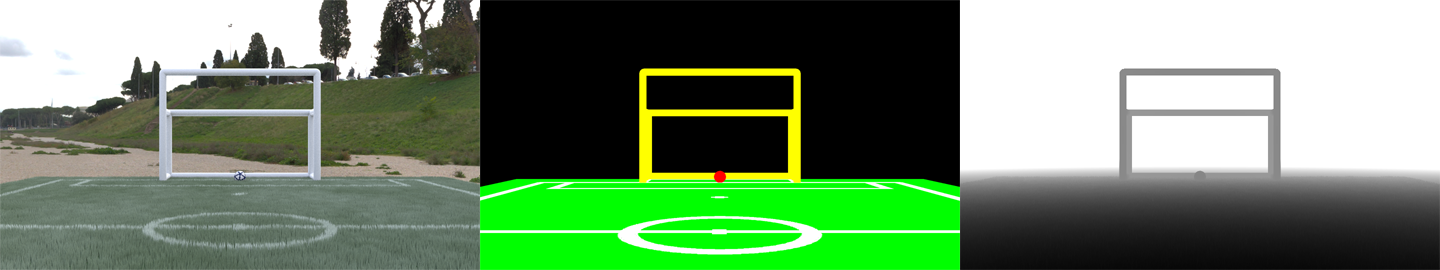
\includegraphics[width=0.99\linewidth]{NUpbr.png}
    \caption{Example outputs of the PBR pipeline, including the raw, segmentation and depth images.}
    \label{fig:pbrExample}
\end{figure}

\noindent\textbf{Adaptive Foot Placement:} 
A dynamic foot controller has been developed by a Mathematics undergraduate student to create a more stable walk engine for the robots. The new controller uses a vector field to dynamically keep the foot on the correct trajectory to the target. Figure \ref{fig:vec_field} shows an example of the vector field that is used to control the motion of the foot. A similar concept was used to develop a dynamic torso controller, which aims at keeping the robot's centre of mass above the robot's support polygon.\\

\begin{figure}[h!]
    \centering
    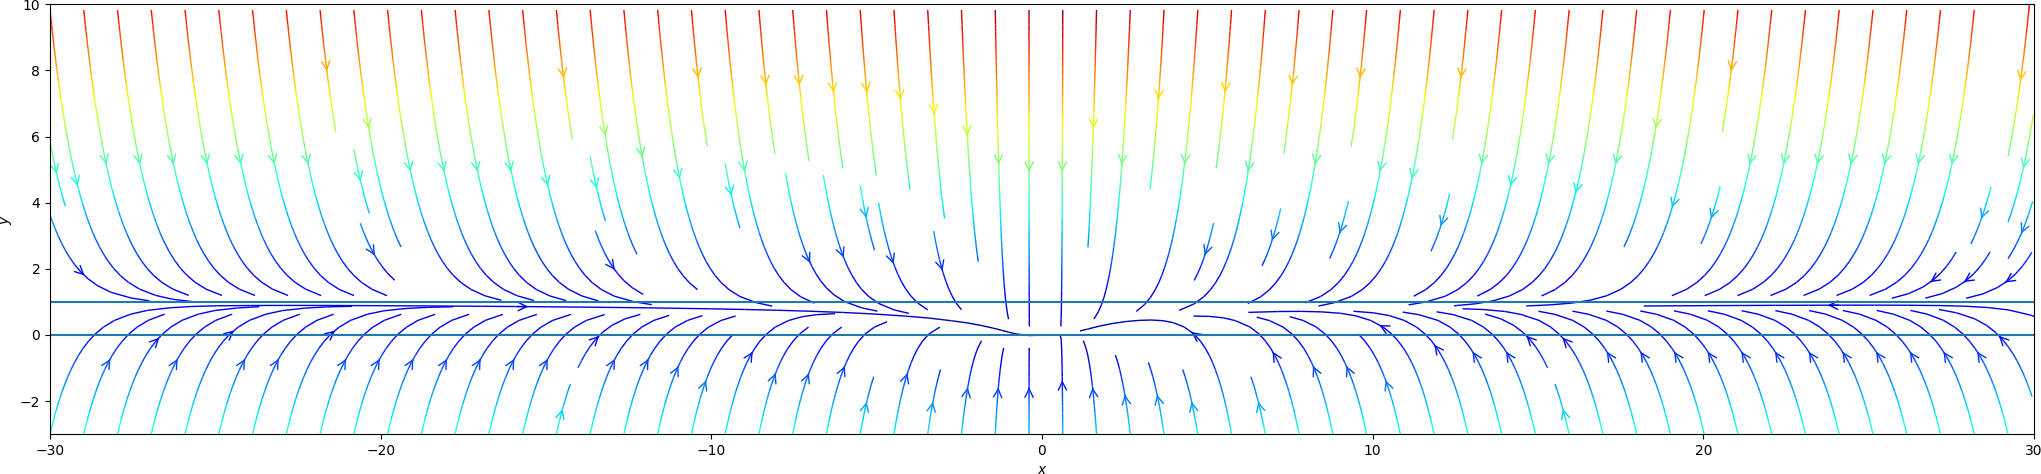
\includegraphics[width=0.99\linewidth]{VectorFieldPlot.png}
    \caption{Vector field of foot step path. Regardless of where the foot is in the vector field it will be pushed to the point $\left(0, 0\right)$.}
    \label{fig:vec_field}
\end{figure}

\noindent\textbf{Advanced Subcontroller Design:} 
Based on comments from other teams at RoboCup 2018 and the NUbots own issues with the CM730 subcontroller, the NUbots have been developing a new subcontroller, dubbed the NUSense. The NUSense is designed to have individual communication busses for up to 6 limbs with individually fused power lines, a 4-cell battery monitor, 2 fan controllers (in case extra internal cooling is required), and a six-axis IMU. Figure \ref{fig:nusense} shows a rendering of the subcontroller PCB, with dimensions of $101.6\times 101.6\textrm{ mm}$. \\

\begin{figure}[h!]
    \centering
    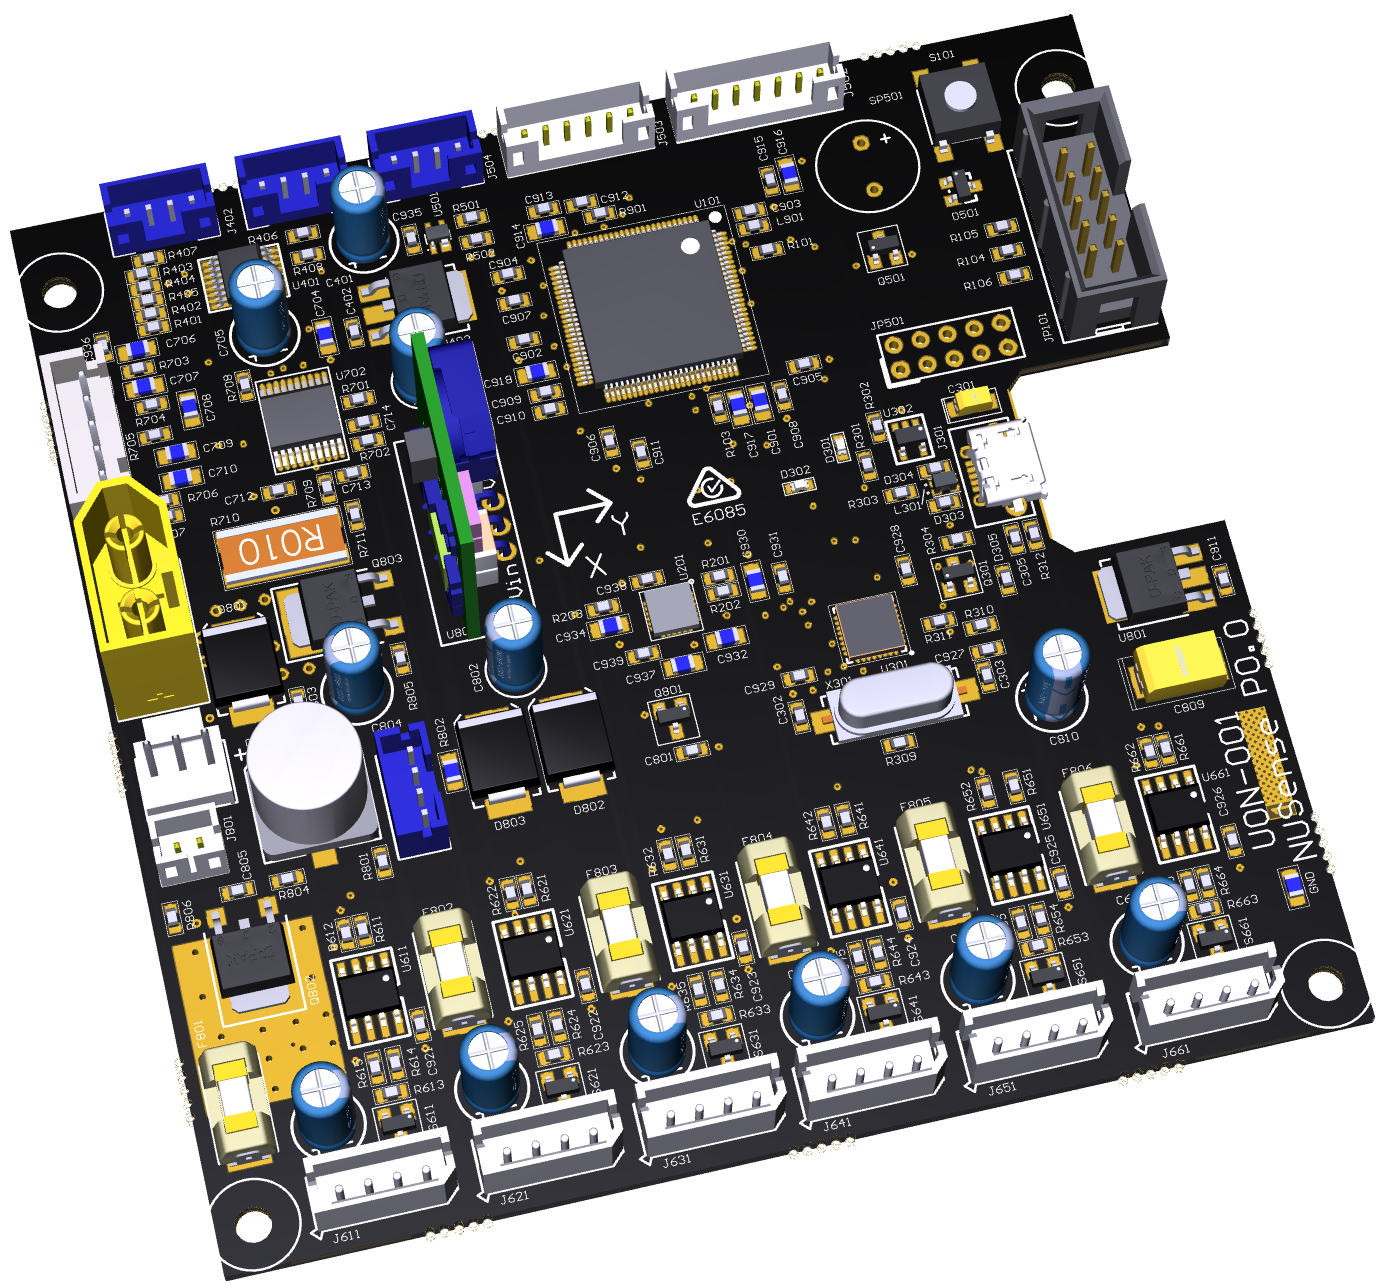
\includegraphics[width=0.80\linewidth]{NUsense3D.png}
    \caption{3D render of the subcontroller PCB. Dynamixel servo connectors are along the bottom edge. The top edge has connectors for LEDs, buttons and fans. The left edge has power connections. In the center is the IMU with its $x$ and $y$ axes marked. On the inset right edge is the USB connection to a PC.}
    \label{fig:nusense}
\end{figure}


\noindent\textbf{Isolated Toolchain Builder:}
A Python-based toolchain builder, named Reel, has been developed to create a toolchain that is completely isolated from the host operating system. This allows the toolchain to be moved to any computer running a Linux-based operating system. The toolchain builder can generate multiple toolchains targeting specific CPUs while also providing a whole host of build tools. \\

\noindent\textbf{Adaptive Script Tuner:}
A new Adaptive Script Tuner is being built in NUsight (a real-time diagnostic/visualisation tool of the robot's operation) to adjust and optimise the motion scripts for the NUbots robots. The new script tuner replaces a basic command-line based script tuner with a visual, web-based GUI that provides real-time feedback when changes are made. It uses a time-based animation system, instead of the previous frame-based system, enabling faster and more intuitive editing of the scripts. \\

\subsection{Background and Research Interests of the NUbots Team Members}

\begin{itemize}
\item \emph{Matthew Amos} is a fifth year undergraduate student studying a combined degree in Computer Science and Computer Engineering with Honours. He is interested in computer vision, machine learning, and synthetic data generation.

\item \emph{Alex Biddulph} is studying for a Doctorate of Philosophy in Computer Engineering. Alex has undergraduate degrees in Computer Engineering and Computer Science with Honours in Computer Engineering. The focus of Alex's studies revolves around the symbiotic relationship between hardware and algorithms, with a focus on high framerate stereo vision for humanoid robots.

\item \emph{Associate Professor Stephan Chalup} is the Head of the Newcastle Robotics Lab. His current research focuses on deep learning, neural information processing systems and topological data analysis.

\item \emph{Daniel Ginn} is pursuing a PhD in Computer Science with a focus on localisation and mapping using robotic platforms in the context of RoboCup. He joined the NUbots competition team in 2017.

\item \emph{Dr. Alexandre Mendes} is the Deputy Head of the Newcastle Robotics Lab. He is a Senior Lecturer in Computing and Information Technology. He joined the group in September 2011 and his research areas are evolutionary algorithms and optimisation.

\item \emph{Josephus Paye} is a third year undergraduate student studying Computer Science, with a major in Computer Systems and Robotics. He contributes to NUsight, the web-based debugging environment.

\item \emph{Ysobel Sims} is an undergraduate student studying a combined degree in Computer Science and Mathematics. She is interested in the mathematics behind humanoid robots, including balance and motion.

\item \emph{Peter Turner} is technical staff in the School of Electrical Engineering and Computing. Peter provides hardware support and assists the team with physical robot design upgrades.

\item \emph{Taylor Young} is a third year undergraduate student studying Electrical Engineering. He contributes to the hardware-based aspects, the design and manufacturing of the robots.

\end{itemize}

The current NUbots team acknowledges the input of team members of previous years and other colleagues from the Newcastle Robotics Lab. Details are linked to  \texttt{www.robots.newcastle.edu.au}.

\subsection{Related Research Concentrations}
The \emph{Interdisciplinary Machine Learning Research Group (IMLRG)} investigates different aspects of machine learning and data mining in theory, experiments and applications. The IMLRG's research areas include: Dimensionality reduction, vision processing, robotics control and learning,  evolutionary computation, optimisation, reinforcement learning, kernel methods, and deep learning. 

\section{History of the NUbots and Prior Performance in RoboCup Competitions \cite{AmosEtAl2018}}
The NUbots team competed in the Four-Legged-League from 2002-2007 using Sony AIBO ERS-210 and ERS-7 robots. The NUbots participated for the first time at RoboCup 2002 in Fukuoka in the Sony Four-Legged League (third place). At RoboCup 2006 in Bremen, Germany, the NUbots won the title.

From 2008 to 2011 they used the Aldebaran Nao within the Standard Platform League. They achieved a first place in 2008 as part of the NUManoid team in Suzhou, China.

The NUbots joined the Kid-Size Humanoid League in 2012 with the DARwIn-OP robots, and ported their SPL codebase to the new platform. They retained their robust and fast vision and localisation systems from the SPL, and ported the B-human NAO walk to the DARwIn-OP for 2012-2013. From 2014-2016 the NUbots redeveloped their software system based on the NUClear software architecture~\cite{HoulistonEtAl2015}. For the DARwIn-OPs, they made small modifications of the head, feet and cameras. In 2017 the NUbots reached the quarter finals of the KId-Size Humanoid League using their mixed team of DARwIn-OP an Igus-Nimbro based robots~\cite{allgeuer2016igus}. After the competition, the team retired all DARwIn-OP robots, replacing them with their NUgus platform; a modified Igus-Nimbro design. In 2018, the NUbots competed in the Teen-Size Humanoid League for the first time using a team of their NUgus robots and finished in third place. In 2019, the NUbots will again compete in the Teen-Size Humanoid League with further improvements to their NUgus design.

%\pagebreak
\section{Software and Hardware Overview}
The NUbots team's software source is available from \cite{nubotsGit} and is covered under the GPL. This code includes associated toolkits for building and deploying the software. Our software is designed to work on multiple robotic platforms, and all of the individual modules have been designed to be easily used in other systems. The flexibility of our approach has been demonstrated in a deployment of the NUbots vision system on a maritime platform\footnote{\texttt{http://www.newcastle.edu.au/about-uon/governance-and-leadership/ faculties-and-schools/faculty-of-engineering-and-built-environment/ maritime-robotx-challenge-team/about-us}}, and the adaptation of the codebase to support both the DARwIn-OP and Igus-Nimbro/NUgus platforms, encompassing both 32-bit and 64-bit CPU architectures with easy adaptability to ARM-based platforms.

Following development of a new software system in 2014-2017, the NUbots are now focusing on the RoboCup Teen-Size Humanoid League. Their research aims include efficient vision processing; improved localisation; generic ball detection; and improving the walk engine. The NUClear based NUbots software is designed to allow new teams and team members to easily understand and innovate on existing code, and is made freely available to encourage research and innovation. Recently, the ability to integrate modules implemented in Python has been incorporated into the NUbots codebase, further increasing the ease for new teams and team members to incorporate their code into the NUbots and NUClear systems.

\section{Enhancements of the NUbots’ Hardware and Software Compared to the Previous Year}
Based on comments from other teams at RoboCup 2018 and the NUbots own issues with the CM730 subcontroller, the NUbots have been developing a new subcontroller, as stated in Section 2.1.

The Gazebo simulation engine was integrated with the NUbots software architecture to facilitate simulation of the robots systems and to enable the use of genetic algorithms and reinforcement learning to find improved solutions to bipedal walking and other necessary humanoid motions.

\subsection{Details on Software and Hardware used from Other Teams}

\subsubsection{Acknowledgement of the use of code for the walk engine:}
The NUbots robots used a walk engine based on the 2013 Team Darwin code release. We acknowledge the source of this code. The NUbots have ported this code to C++ and restructured the logic, making numerous structural and technical changes. The current code for the NUgus robot walk is a further modification and extension of the code that the NUbots used on their Darwins in previous years.

\subsubsection{Acknowledgement of the use of robot design files:}
The NUbots NUgus robots are based on the 2016 Team Nimbro design files~\cite{igusDesignFiles}. We acknowledge the source of this design. The NUbots have made modifications to the design to account for a different printing process and to improve the usability of the design. The modified design files are released under the original license~\cite{nubotsHardwareGit}.

\subsubsection{The NUbots team’s own contributions:}
The NUbots vision system now utilises the Visual Mesh algorithm~\cite{Houliston2018VisualMR}. This algorithm allows for fast, efficient, and accurate deep learning to be performed on high resolution images at frame rates in excess of 400 frames per second. The implemented algorithm provides guarantees over the number of sampled pixels within a given object and at any distance from the camera, allowing the user full control over the trade-off between the algorithms run time and accuracy.

\subsection*{Acknowledgement} The NUbots team is grateful to their main industrial partners and sponsors 4Tel Pty Ltd, Tribotix, Pritchard Electronics and the Morris Group. They also would like to thank the School of Electrical Engineering and Computing, and the Faculty of Engineering and Built Environment at The University of Newcastle, Australia, for their continuous support. Alex Biddulph is supported by an Australian Government Research Training Program scholarship and a top-up scholarship through 4Tel Pty Ltd.


\bibliographystyle{plain}
% argument is your BibTeX string definitions and bibliography database(s)
\bibliography{nubots}

\end{document}
